\documentclass[11pt]{article}
\usepackage[letterpaper,margin=0.85in]{geometry}
\usepackage[T1]{fontenc}
\usepackage[utf8]{inputenc}
\usepackage{lmodern}
\usepackage{microtype}
\usepackage{graphicx}
\usepackage{amsmath}
\usepackage{parskip}
\usepackage{fancyhdr}
\usepackage{hyperref}
\hypersetup{hidelinks,pdftitle={Attempt at a Mathematical Theory of the Coagulation Kinetics of Colloidal Solutions}}
\pagestyle{fancy}
\fancyhf{}
\fancyhead[L]{M. von Smoluchowski (1917)}
\fancyhead[R]{Literal English translation}
\fancyfoot[C]{\thepage}
\setlength{\headheight}{14pt}
\title{Attempt at a Mathematical Theory of the Coagulation Kinetics of Colloidal Solutions}
\author{M. von Smoluchowski}
\date{Received September 8, 1916; published 1917\\[1ex]\small Literal English translation from the attached German scan}
\begin{document}
\maketitle
\begin{center}
\emph{With 8 figures in the text}
\end{center}
\noindent\textbf{Translator's note.} This edition follows the supplied scan page by page and preserves the author's terminology, numbering, references, and historical wording. Source-page headings refer to the original journal pagination (pp.~129--168). A facsimile of each source page follows its English rendering so that equations, tables, and uncertain scan characters can be checked directly.
\tableofcontents
\clearpage
\section*{Verified mathematical transcription}
\addcontentsline{toc}{section}{Verified mathematical transcription}
\noindent The equations below have been transcribed directly from the printed facsimile. Equations (30)--(32), absent from the supplied scan because journal pages 158--159 are missing, have been recovered from Smoluchowski's manuscript. These displays supersede any equation-like OCR fragments in the page-by-page prose transcription.

\begin{align}
D&=\frac{H\Theta}{N}\frac{1}{6\pi\mu a},\tag{1}\\
W(x)\,dx&=\frac{1}{2\sqrt{\pi Dt}}\exp\!\left(-\frac{x^2}{4Dt}\right)dx,\tag{2}\\
\overline{x^2}&=2Dt,\tag{3}\\
\frac{\partial(ru)}{\partial t}&=D\frac{\partial^2(ru)}{\partial r^2},\tag{4}\\
u&=c\left[1-\frac{R}{r}+\frac{2R}{r\sqrt{\pi}}
\int_0^{(r-R)/(2\sqrt{Dt})}e^{-z^2}\,dz\right],\tag{5}\\
J\,dt&=4\pi DR^2\left.\frac{\partial u}{\partial r}\right|_{R}dt
=4\pi DRc\left(1+\frac{R}{\sqrt{\pi Dt}}\right)dt,\tag{6}\\
M&=\int_0^tJ\,dt=4\pi DRc\left(t+\frac{2R\sqrt t}{\sqrt{\pi D}}\right),\tag{7}\\
W_t&=\frac{4\pi DR}{V}\left(t+\frac{2R\sqrt t}{\sqrt{\pi D}}\right),\tag{8}\\
U_t&=\exp\!\left[-4\pi DRv_0\left(t+\frac{2R\sqrt t}{\sqrt{\pi D}}\right)\right],\tag{9}\\
w&=4\pi DRv_0,\tag{10}\\
v_1&=v_0e^{-4\pi DRv_0t},\tag{11}\\
-\frac{dv_1}{v_1}&=4\pi DRv_0\,dt,\tag{12}\\
\frac{1}{v_1^2}\frac{dv_1}{dt}&=-4\pi DR,\tag{13}\\
v_1&=\frac{v_0}{1+4\pi DRv_0t}=\frac{v_0}{1+t/T},\tag{14}\\
T&=\frac{1}{4\pi DRv_0},\tag{15}\\
v_1&=\frac{v_0}{1+8\pi DRv_0t}=\frac{v_0}{1+2t/T}.\tag{16}
\end{align}

\begin{align}
\frac{1}{4\pi}\frac{dv_1}{dt}
 &=-D_{11}R_{11}v_1^2-D_{12}R_{12}v_1v_2-D_{13}R_{13}v_1v_3-\cdots,\tag{17.1}\\
\frac{1}{4\pi}\frac{dv_2}{dt}
 &=\tfrac12D_{11}R_{11}v_1^2-D_{12}R_{12}v_1v_2-D_{22}R_{22}v_2^2-D_{23}R_{23}v_2v_3-\cdots,\tag{17.2}\\
\frac{1}{4\pi}\frac{dv_3}{dt}
 &=D_{12}R_{12}v_1v_2-D_{13}R_{13}v_1v_3-D_{23}R_{23}v_2v_3-\cdots,\tag{17.3}\\
\frac{1}{4\pi}\frac{dv_4}{dt}
 &=\tfrac12D_{22}R_{22}v_2^2+D_{13}R_{13}v_1v_3-D_{14}R_{14}v_1v_4-\cdots.\tag{17.4}
\end{align}
\begin{align}
R_{ik}&=\tfrac12(R_i+R_k),\notag\\
D_{ik}R_{ik}&=\tfrac12(D_i+D_k)(R_i+R_k)
=\frac{DR}{2}\frac{(R_i+R_k)^2}{R_iR_k},\tag{18}\\
4\pi D_{ik}R_{ik}&=8\pi DR=2\alpha.\tag{19}
\end{align}

\begin{align}
\frac{1}{2\alpha}\frac{dv_1}{dt}&=-v_1^2-v_1v_2-v_1v_3-v_1v_4-\cdots,\notag\\
\frac{1}{2\alpha}\frac{dv_2}{dt}&=\tfrac12v_1^2-v_1v_2-v_2^2-v_2v_3-\cdots,\notag\\
\frac{1}{2\alpha}\frac{dv_3}{dt}&=v_1v_2-v_1v_3-v_2v_3-v_3^2-\cdots,\tag{20}\\
\frac{1}{2\alpha}\frac{dv_4}{dt}&=\tfrac12v_2^2+v_1v_3-v_1v_4-v_2v_4-\cdots,\notag\\
v_1+v_2+v_3+v_4+\cdots&=\sum v,\tag{21}\\
\frac{1}{2\alpha}\frac{dv_1}{dt}&=-v_1\sum v,\notag\\
\frac{1}{2\alpha}\frac{dv_2}{dt}&=\tfrac12v_1^2-v_2\sum v,\notag\\
\frac{1}{2\alpha}\frac{dv_3}{dt}&=v_1v_2-v_3\sum v,\notag\\
\frac{1}{2\alpha}\frac{dv_k}{dt}
 &=\tfrac12\left(v_1v_{k-1}+v_2v_{k-2}+\cdots+v_{k-1}v_1\right)-v_k\sum v.\tag{22}
\end{align}

\begin{align}
\sum v&=\frac{v_0}{1+\alpha v_0t}=\frac{v_0}{1+4\pi DRv_0t}=\frac{v_0}{1+t/T},\tag{23}\\
v_1&=\frac{v_0}{(1+\alpha v_0t)^2}=\frac{v_0}{(1+t/T)^2},\notag\\
v_2&=v_0\frac{\alpha v_0t}{(1+\alpha v_0t)^3},\qquad
v_3=v_0\frac{(\alpha v_0t)^2}{(1+\alpha v_0t)^4},\notag\\
v_k&=v_0\frac{(\alpha v_0t)^{k-1}}{(1+\alpha v_0t)^{k+1}},\tag{24}\\
\frac1T&=4\pi DRv_0=\frac1t\left(\sqrt{\frac{v_{10}}{v_1}}-1\right),\tag{25}\\
\frac{R}{r}&=\frac{N}{H\Theta}\frac{3\mu}{2v_0}\frac1T,\tag{26}\\
T&=\frac34\frac{N\mu}{H\Theta\varepsilon v_0},\tag{27}\\
\beta&=\frac{1}{6\pi}\frac{\partial u}{\partial x}\frac{R^2}{D}
=\frac{4r^3\mu}{H\Theta/N}\frac{\partial u}{\partial x},\tag{28}\\
\lim y&=1-\left(1+\frac1x\right)e^{-1/x},\qquad x=\frac{t}{T}.\tag{29}
\end{align}

\begin{align}
\frac{dx}{dt}&=kt(1+bx)(1-x)^2
\quad\text{or}\quad
\frac{dx}{dt}=k't(1+b'x)(1-x),\tag{30}\\
\frac{dx}{dt}&=k_1(1+b_1x)(1-x),\tag{31.1}\\
\frac{dx}{dt}&=k_2(1+b_2x)(1-x)^2,\tag{31.2}\\
\frac{dx}{dt}&=k''(1-x)^2,\tag{31.3}\\
\mu&=\mu_0\left(1+\frac52\varphi\right),\tag{32}\\
\mu&=F\!\left[v_0\Phi(v_0t)\right],\tag{33}\\
F&=\mu=\mu_0\left(1+0.198\varphi+0.069\varphi^2\right),\tag{34}\\
\Phi&=0.131+0.869\left(\frac{\vartheta}{\vartheta+3.94}\right)^3,\tag{35}\\
\Phi&=\omega+\sigma\left(\frac{t}{t+T}\right)^3.\tag{36}
\end{align}

\clearpage

\section*{Source page 129}
\addcontentsline{toc}{section}{Source page 129}
\_ Attempt at a mathematical theory of the coagulation kinetics of colloidal solutions.

From

M. von Smoluchowski. (With 8 figures in the text.) (Received September 8, 1916.)

I. Introduction.

So does the literature on coagulation to this day. colloidal solutions have grown, our knowledge of the quantitative course and the mechanism of the coagulation process is extremely inadequate. Most researchers content themselves with qualitative observations or present their series of measurements in tables or curves, since the mathematical reproduction of these encounters exceptional difficulties.

In the interesting works?) by S. Miyazawa, N. Ishizaka, H. Freundlich, J. A. Gann, however, a formulaic summary of the empirical experimental material is sought, as well as an elucidation of it by analogy with the laws of chemical kinetics. But clear chains of laws have not yet emerged in this way, and certain law formulas that were initially established (Paine, Freundlich and Ishizaka) were even used by closer examination (Freundlich and Gann) withdrawn as untenable ').

The failure of previous attempts to gain an understanding of the laws that apply here by empirical-inductive means can now be seen as a reason to consider the circumstance

1) Cf. e.g. B.: A, Galecki, Zeitschr. f. anorg. Chemistry 74, 174 (1912); Colloid Magazine 10, 169 (1912); A. Lottermoser, Colloid Journal. 15, 145 (1914); H. H © Paine, Colloid Chem. Supplements 4, 24 (1912); Colloid Magazine 11, 115 (1912). . .

4) 8. Miyazawa, Journ. Chem. Soc. Tokyo 83, 1179, 1210 (1912); N. Ishizaka,

Magazine f. physics. Chemistry 88, 97 (1913); H. Freundlich and N. Ishizaka, there

. 85, 398 (1918); Colloid Magazine 12, 230 (1913); J. Gann, Colloid Chem. Supplements 8,

64 (1916). \_ 8) See Section VI. Tent writing for physics. Chemistry. XCIf, 8

\clearpage
\begin{center}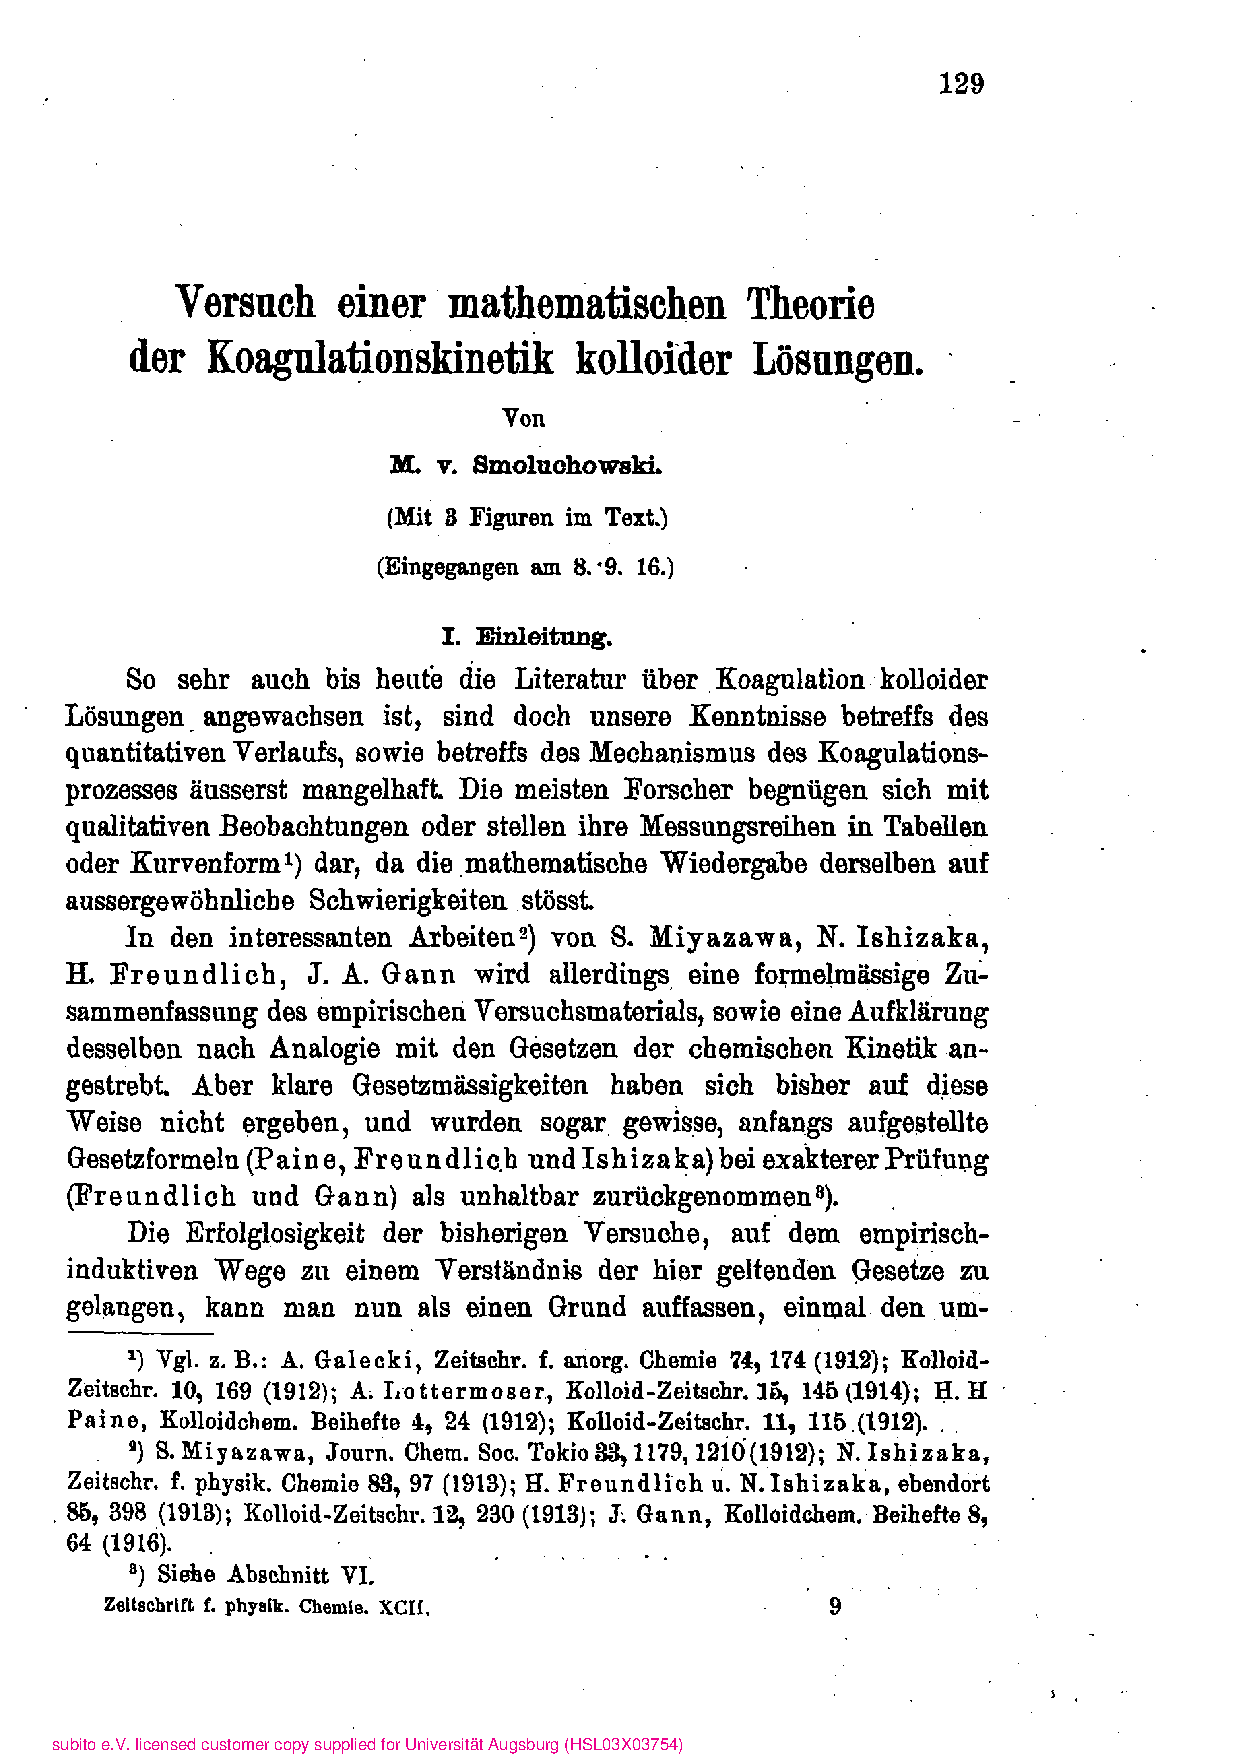
\includegraphics[page=1,height=0.94\textheight]{Smoluchowski-Koagulation_1917.pdf}\end{center}
\clearpage
\section*{Source page 130}
\addcontentsline{toc}{section}{Source page 130}
130. M, v. Smoluchowski

to take the inverted, deductive path and - however daring it may be
given the ignorance of the internal mechanism of coagulation
may seem - to at least work out certain theoretical guiding principles that will provide a clue when working on this area
could give. The following is such a theoretical scheme
the coagulation kinetics are developed!), which I as a result of a
Prof. R. Zsigmondy's suggestion was developed when he was in the
In the course of his investigations into coagulating gold solutions to me
wrote a letter asking whether, on the basis of a certain,
The idea that still needs to be discussed is a mathematical theory
of these phenomena could develop.

But of course this theory doesn't want to happen all at once
provide a definitive explanation of the entire coagulation problem, but rather
'For the time being, it only aims at a mathematical formulation of the
mechanism of this phenomenon that is accessible to immediate observation.
First and foremost, the limiting case of "rapid" coagulation examined by Zsigmondy is taken into account, which corresponds to a complete discharge of the colloid particles as a result of a large amount of electrolyte. However, it seems to me that this theory is in
‘little modified form even on slow ones (through incomplete ones
Discharge induced) coagulation can be transmitted and that it
should provide a means of partially solving the complicated processes of this kind
to unravel and the previously mentioned experimental studies
theoretically”. utilize,

This brings us back to the question of why the empirical-inductive method has not yet led to any real success. I
I believe that this is largely due to a fact of fundamental importance: that in almost all previous work certain dimensions,
such as toughness, relative amount of under certain conditions in
Substance in solution, light permeability, was considered a measure of coagulation, while in reality it is not an exact one
“Measure of coagulation” in that the latter does not undergo any coagulation at all
display only one variable. Those measurable sizes depended
in an extremely complicated and largely unknown way of various variables, namely both in number and in terms of
the size, shape, structure of the colloid particles and gradually
'forming aggregates, and it is not possible the other way around.

4) I found the main results in a conference organized by the Wolfskehlstiftung
Lecture cycle in Géttingen, June 20-22, announced; see physics. Magazine 1\%,
557, 685 (1916).

\clearpage
\begin{center}\includegraphics[page=2,height=0.94\textheight]{Smoluchowski-Koagulation_1917.pdf}\end{center}
\clearpage
\section*{Source page 131}
\addcontentsline{toc}{section}{Source page 131}
Attempt at a mathematical theory of coagulation kinetics etc. 131

The resulting overall effect draws clear conclusions about the partial
\_ to draw events.
One cannot expect simple and general laws either
for those quantities such as the vapor pressure and the force
or the optical properties of a liquid, which consists of several,
Components that react chemically with each other are mixed:
In the latter case, additional laws only exist for: the
changes in the number of molecules; they are also with the. Coagulation
only for the changes in the numbers of particles. certain
Genera are to be expected, not for the overall changes in certain physical properties caused by this. From this point of view, only direct payments of the particles (of the various categories) made at certain time intervals, such as those according to Zsi gmondys, should be considered as rational experimental material
Methods can be carried out on colloidal gold solutions \}). oe
« Unfortunately, the applicability of this is currently limited to a few such cases and is associated with considerable experimental difficulties. But Zsigmondy has recently managed to get his
methods, which he will report on in more detail elsewhere, and it is to be hoped that in the future. these
In this way, a more extensive, precisely defined test material is obtained
will be. Preliminary measurements, kindly communicated by Zsigmondy
will also serve as the first touchstone for our theory in what follows
form, and we will see that they are the same in a more satisfactory way
way. It will also be proven that the
\_ Main results of previous work in it a complete explanation
find. This justifies the hope that they will also be successful in further ones
such studies, at least as a preliminary guide
will prove. -

Il. Physical foundations of the coagulation theory.

Despite all the effort put into these investigations, there is a lack
there is still a clear knowledge of the effective causes,
which require stability or coagulation, and it seems difficult to
decide which of the diverse ideas advocated by colloid researchers should be used as the basis for theoretical treatment

1) Similar payments are to show the coagulation process of
J. Reissig [Ann. d. Phys. 27\%, 186 (1908)] and especially by A. Galecki
[Zeitechr. f. anorg. Chemistry 74, 174 (1912); Colloid Magazine 10, 169 (1912)]

been led. We will come back to these in Section IV.
:g*

\clearpage
\begin{center}\includegraphics[page=3,height=0.94\textheight]{Smoluchowski-Koagulation_1917.pdf}\end{center}
\clearpage
\section*{Source page 132}
\addcontentsline{toc}{section}{Source page 132}
132 m.v. Smoluchowski

have to choose. That's why we have to think about these questions first and foremost
form a judgment.

One thing is probably generally recognized today, that the coagulation
-lating effect of the electrolyte additive on irreversible hydrosols
based on an electrical phenomenon, which is caused by the same
caused by electrosmotic and cataphoretic phenomena
known reduction in particle charge goes parallel and is actually closely related.

Hardy), who first noticed this connection, wanted
ibn through a protective effect of the electrical double layer
Particles explain that the sinking of the particles is cataphoretic
"Dornian" currents would have to excite, which would have to counteract the movement. Undoubtedly such an effect actually exists, but
is it practically out of the question?); at all the fall is on
which this theory refers to is obviously only a secondary process,
the primary cause of this would be the agglomeration of the particles
but remain unexplained.

Billiter® sees coagulation as a direct electrostatic charging effect of the ions on the charged particles. So simple
But the mechanism certainly cannot be, because the specific differences in the effectiveness of different ions become inexplicable.
In view of the differences in mobility, the
Clays attach to the particles and not the other way around, and it would have to
Electrical double layers are created there - if they don't already exist
hiften existed from the start. |

. It should be emphasized that the “particle charges”
not, as so often happens, as isolated electrostatic charges -
according to the type of charge of fog droplets in air - can be imagined, since the
Particles are embedded in an electrolytically conductive medium.
What is called “particle charges” for short is the charge on the inner coating of the electrical double layer, which passes through in the resting state
the opposite ionic layer in its effect towards the outside
is compensated; Movement processes only occur at the same time
Shifting of the two double-layer occupancies occurs. Given

1) W. B. Hardy, magazine. f. \_physics. Chemistry 33, 885 (1900); Proc. Roy. Soc.
66, 110 (1900).

*) See M. v. Smoluchowski, Krak. No. 1903, p. 182; and d. Article “Electrical Endosmosis and Current Flows” in Graetz’s Handbook d. Electric, II 2

(1914) 8. 420.
- 5) J. Billiter, Journal. f. physics. Chemistry 45, 307 (1908); 48, 513, 542 (1904)

51, 128,-167 (1905).

\clearpage
\begin{center}\includegraphics[page=4,height=0.94\textheight]{Smoluchowski-Koagulation_1917.pdf}\end{center}
\clearpage
\section*{Source page 133}
\addcontentsline{toc}{section}{Source page 133}
Attempt at a mathematical theory of coagulation kinetics etc. 133

the extensive quantitative agreement of the electrosmotic
and cataphoretic phenomena with Helmholtz's double layer theory, which is one of the few confirmed results
In this area, one does not get this theory without compelling reasons
Reason leave dirfen.

This also means that the theory is untenable. Hatsheks’)
proven, according to which the stability of the colloid@ is an effect of the
electrostatic, simply calculated according to Coulomb's law 2u, repulsion of the particle charges wire, thus according to the measure
as the discharge of the particles progresses. Obsess
Each particle of a colloidal oil-water emulsion has a free charge
from the order of magnitude 44-10-7 electrostatic purity - namely
without a compensating countercharge, as Hatschek apparently assumes -,
This is how a drinking glass would be full of such a massively concentrated drink
Solution (3-10!° particles per cc) there are already charges of the order of 10° increments, which immediately attack the simple particles
the externals are driving and in general quite colossal on the outside
would have to exert electrostatic effects. There is no trace of this
It should be noted that the solution behaves externally in its normal state
electrically neutral. -

The assumption of electrostatic long-distance forces acting across the particle distance is certainly untenable, and we need force effects
assume that this only becomes noticeable when the particles approach directly
become.

According to Bredig?) it is a phenomenon that...
Changes in the surface voltage of mercury due to polarization are analogous; The cause of coagulation is capillary forces
reach a maximum in the isoelectric point. Then it would have to be there
However, the coagulation speed can be the highest, but the
The stability of the solutions below the threshold value of the electrolyte concentration is incomprehensible. R. Ellis also found this with oil emulsions
no connection with the surface tension; if so
Capillary forces certainly play an important role in these processes
as the connection cannot be direct.

Freundlich expressed other thoughts. Accordingly

*) E. Hatschek, Colloid Journal. 9, 159 (1911).

*") G. Bredig, Anorg. Ferments 1901.

*) Ridsdale Ellis, magazine. f. physics. Chemistry 78, 321 (1911).

*) H. Freundlich, Capillary Chemistry 1909, pp. 261, 347; timeline f. physics.
Chemistry 73, 385 (1910). H. Paine has this idea in a slightly different way

\clearpage
\begin{center}\includegraphics[page=5,height=0.94\textheight]{Smoluchowski-Koagulation_1917.pdf}\end{center}
\clearpage
\section*{Source page 134}
\addcontentsline{toc}{section}{Source page 134}
134. So M. v. Smoluchowski...- 85-5 0h ;

The coagulation is caused by accidental charge asymmetries and corresponding potential differences in the particles, which are the case
Collision of the latter results in a breaking through of the separating viscous
Fluid layer should be favored, similar to (according to experiments
by Lord Rayleigh and Kaiser) the union of water jets,

\_ Droplets, soap bubbles, etc. are accelerated by applying relatively small potential differences.

Z. The cause of the latter process is obviously the accumulation of very significant opposite charges on the two
To look for occupancies in the thin separating air layer, which generates significant pressure forces that accelerate the breaking through of the latter
can cause. Analogous attractive effects then come about
expect a sign change as soon as the random asymmetries occur
of the charges would require, i.e. i. in the immediate vicinity of the
isoelectric point, while according to Powis z. B, olemulsions do

- then begin to coagulate when the potential difference of the double layer is still 0-03 volts, i.e. in relation to the normal value
0-046 volts has only decreased by a third). Differences in
The size of the charge does not in itself imply any tendency towards unification as long as the sign is the same, just like
There is not the slightest effort between monovalent and polyvalent cations
an association exists.

Furthermore, it seems to me that the dissipative toughness resistance
the separating air or liquid layer, which was in the previous
The phenomena mentioned only come to light in kinetic processes
role, but not for the conditions of a static equilibrium?) can be decisive, as this undoubtedly exists at least in the case of reversible colloids (e.g. Sven Odén's sulfur solutions).
So stability and coagulation ability can have nothing to do with it.

- The simplest assumption is perhaps that the particles
with sufficient approximation as a result. the capillary forces attract; that
but a union does not occur under normal circumstances, wire
due to a protective effect of the electrical double layer,
which can be visualized in the manner of a rubber pad.
When electrolytes are added, this occurs as a result of what was demonstrated by Freundlich

' recorded: Colloid Magazine. 11, 119 (1912). See also H. Freundlich and.
N. Ishizaka, Colloid Journal. 12, 235 (1913).
) F. Powis, Journal. f. physics. Chemistry 89,186 (1914).
3) Zabigkeit not only counteracts the approach of two particles,
but. as well as their removal.

\clearpage
\begin{center}\includegraphics[page=6,height=0.94\textheight]{Smoluchowski-Koagulation_1917.pdf}\end{center}
\clearpage
\section*{Source page 135}
\addcontentsline{toc}{section}{Source page 135}
Attempt at a mathematical theory of coagulation kinetics etc. 135

Ion adsorption involves a partial or complete discharge of the double layer, which reduces its protective effect. that same
from a certain level of concentration onwards it is no longer sufficient,
to prevent the parts from colliding and sticking together. . Thu |

In 'Gummiguttlésungen Costantin and: 'Perrin\}) in: whole .
precisely proven that their particles (radius 0-33 «) under
under normal circumstances are surrounded by a repulsion sphere of the order of magnitude of 1-7 times the particle radius. It is to be expected that these will decrease with the addition of electrolytes and eventually
will give way to a sphere of attraction. If the rubber solution is slightly acidified (almost 0-01-norm.), then they remain
Particles stick to the glass wall as soon as they come into contact with it; will
If they become more acidic, they also unite with each other
Aggregates as soon as they come into contact. The “adagulation”.
the glass wall, which one from L. Brillouin?) to demonstrate diffusion
has been used, I consider it to be one of coagulation exactly | corresponding one-dimensional process.

With all this comes. Of course, apart from those force effects
a third factor comes into consideration, which on the one hand is a collision -
of the particles, but on the other hand their permanent union
counteracts, namely the molecular agitation, which, among other things
as Brownian motion. But this factor is like that
Statistical mechanics teaches that a constant (i.e. at a certain -
Colloid only depends on the temperature, but otherwise on no other circumstances) size, which is therefore suitable for the electrolyte addition
The Boagulathon tendency caused by this should not be held responsible -
that can. © ; |

By the way, it has been directly experimentally proven by Svedb: ergs measurements that: the intensity. Brownian motion is not influenced by the addition of electrolytes. She changes
only secondary, corresponding to that produced by coagulation
Size growth of the particles being observed.’ So
The untenability of those theories that attribute coagulation to changes in Brownian motion has also been proven.

J, Perrin, Compt. rend...158, 1168 914); R, Costantin,- Compt rend.
158, 1171, 1341 (1914). |

" 4) Anne. Chim. Phys. 2\%) 412 (1912). Vel: also M. v. Smoluchowski, Vienna.
Ber, 124, 263 (1915) and the Gdttingen report mentioned at the beginning. 6
8) The Svedberg, The existence of molecules, 1912, -p. 105."

\clearpage
\begin{center}\includegraphics[page=7,height=0.94\textheight]{Smoluchowski-Koagulation_1917.pdf}\end{center}
\clearpage
\section*{Source page 136}
\addcontentsline{toc}{section}{Source page 136}
136 ; M.v. Smoluchowski

This also refers to N. Pappada's considerations'), according to which

the collisions of the diffusing ions inhibit the Brownian
movement and thereby cause coagulation. that,
As Pappada found, the effectiveness of the monovalent inorganic ions parallels their migration speed, is -
certainly a very interesting fact, but it proves nothing for those
somewhat unclear theory at all; As is well known, molecular kinetics teaches that the kinetic energy of all anions, cations and neutrals
Molecules are the same size and the differences in migration speeds are based on a completely different circumstance: the differences in size of the ions (including water shells) and their different
Movement resistance.

Our statements so far should be sufficient to make the basic assumption*) of the theory presented below plausible.
This is the case of complete particle discharge
coagulation occurs, we want to assume that every particle is surrounded by a certain sphere of attraction, so that a
second particle carries out its Brownian motions undisturbed,
as long as it is outside that area, but for .
always united with that one as soon as it came into its area. It
So the undoubtedly continuous transitions are carried out by one
discontinuous jump replaced; This is unlikely to result in any significant deviations, while on the other hand it will
mathematical considerations are very simplified, since then it no longer exists
on the size and distribution of forces, but only on the size of the
Attraction area arrives.

The problem of the internal mechanism of the attraction forces
Find out to what extent they are capillary or electrical in nature, like them
related to the adsorption of the ions, etc., are not touched upon here. Their solution remains more experimental
Work and a future theory of electrical double layers
reserved. So it becomes a provisional theory in a certain sense
formulated, which is only a first step towards the final solution,
but that doesn't make it any less justified. We talk in a very similar way
in the gas theory of molecular and atomic radii and use them

1) Vel. e.g. B. N. Pappada, Colloid Journal, 9, 265 (1911).
\#) As mentioned, the same was first sent to me in a letter from R, Zsigmondy
- beaten; I readily agreed with this idea because it was completely...
corresponds to my own views and seems to be a description of the facts that contains only a little hypothetical.

,

,

\clearpage
\begin{center}\includegraphics[page=8,height=0.94\textheight]{Smoluchowski-Koagulation_1917.pdf}\end{center}
\clearpage
\section*{Source page 137}
\addcontentsline{toc}{section}{Source page 137}
Attempt at a mathematical theory. the coagulation kinetics etc. 137

- Terms with advantage, although molecules and atoms are certainly not spheres
but are complicated structures made up of electrons and “nuclei”.

III. Mathematical theory of rapid coagulation.

The theory of the double layer at volistindige discharge).
In the following, the occurring, in short, “rapid” coagulation will be discussed
be expanded under the assumption that it is a
Colloidal solution, which originally consists of nothing but equal sizes,
consists of spherical particles, the number of which per unit volume is »,
be referred to. As a result of the electrolyte addition, which should be as instantaneous and uniform throughout the liquid as possible
at time ¢= 0 every particle has a sphere of attraction
of radius R. From now on, its Brownian molecular motions will only remain undisturbed until that point in time
normally carried out where - precisely as a result of those movements -
the center of another particle enters its sphere of attraction. From this moment on, the pair in question is supposed to form an indivisible whole as a result of being put together, which continues its Brownian movements at a reduced speed corresponding to the increase in volume. Through affiliation
of another primary particle to the double particle can be done with the
Time a triple, by union of two doubles or one
triple and a simple a quadruple particle arise, and
in this way the coagulation process would progress until
the entire divided substance has been transformed into a coherent mass if gravity had not previously caused sedimentation of the aggregates.

The mathematical problem to be read consists of calculation.
of the numbers v,, »,, »; ... of the currently existing single, double, triple ... particles, due to the. Indication of the sizes,
which characterize the entire system, namely the original one
Number »,, the size of the radius of action \# and the speed constant D of the Brownian motion.

Certain conclusions can now be made without special calculations,
based solely on the facts that the coagulation report
should be a function of those three sizes. From the diagram of dimensions: \%\textasciitilde{}w 178; Rwl; Dw lt-! you can see that the

1) Experimentally, this limit case is characterized by the features discussed in Section IV.

\clearpage
\begin{center}\includegraphics[page=9,height=0.94\textheight]{Smoluchowski-Koagulation_1917.pdf}\end{center}
\clearpage
\section*{Source page 138}
\addcontentsline{toc}{section}{Source page 138}
BB a ee ML vy. Smoluchowski

Size D is the only one that is related to the time scale.
Since the latter is on the. absolute coagulation process has no influence
can have, it must necessarily have a mere function
of the product (Dz). As a result, the — given »,
and R — to achieve a certain stage of coagulation
required time period is inversely proportional to the diffusion constant
D be.
This can also be used to estimate the influence of temperature
if one assumes what the experimental results regarding de
Size R (see the next section) suggests that the effective radius £ is independent of the temperature. It should then be the coagulation time with reference to the formula?):

HO1
D> OW tama @)
proportional to the ratio \& vary. So you will be at temperature

change approximately proportional to the viscosity of the medium, which is in
There is agreement with some preliminary experiments carried out by Zsigmond y in this regard.

By now moving on to the real calculation, we want
first consider a simplified task by imagining
one of the particles is held and only this one has one
Sphere of attraction, while the other particles do not interact with each other at all
coagulate. |

Under these circumstances, what is the probability that...
until the time ¢ a particle has attached to the highlighted one?

The easiest way to answer this question is on the basis of equivalence
Brownian motion and the diffusion mechanism
lésen2), The process that is called diffusion is namely in
Simply the resulting overall effect of the Brownian motions. of the individual particles. Each one moves independently
from the rest, according to the distribution formula: '

2

Wade = \_

—\_\_\_\_\_..-. @4Dtday. 2

\textbackslash{} 2VxDi Pt 2)
which indicates the probability with which a particle emanating from the zero point reaches an abscissa x... + dx in time t,

1) Exceptionally in this one. Work the absolute temperature is denoted by 0 to avoid the ambiguity with the coagulation time.
2) Relevant details in the Gottingen lectures mentioned at the beginning.

\clearpage
\begin{center}\includegraphics[page=10,height=0.94\textheight]{Smoluchowski-Koagulation_1917.pdf}\end{center}
\clearpage
\section*{Source page 139}
\addcontentsline{toc}{section}{Source page 139}
Attempt at a mathematical theory of coagulation kinetics etc. 139

and it is easy to prove mathematically that these movements
on average to equalize the concentration differences
drive, which is in complete agreement with the usual diffusion theory.
This turns out to be the coefficient D, which is also known in the
Equation for the average displacement square occurs:
m= 2Dt (3)
as identical to the diffusion coefficient of the swarm of parts;
In the case of spherical particles, its value is determined by Einstein's formula (1), which we still use later
become. .
\textasciitilde{} The requirement that the spherical surface of radius R each
We can obviously replace the idea that the incoming particles hold on with the assumption that it has a completely “adsorbing” effect, i.e. that
The concentration zero is maintained at the spherical surface R. As a result, a concentration gap arises in the
Surroundings of the sphere, and in the period ¢...¢-+dé through the
Surface corresponds to the substance diffusing through the latter
exactly the average number of particles that result from them
Brownian motions hit the ball during that period and
be adsorbed. e
However, the equivalence of these two sizes only applies as long as
This "average number" is very small in relation to the number, otherwise there is the possibility of simultaneous adsorption of several
Particles came into consideration, which would have to proceed differently due to their mutual interference. The equivalence is certainly valid,
if the number », is sufficiently small; therefore we take it for the time being
assume it is about. the probability of adsorption of a
single particle present somewhere within the extremely large volume V. |
Now the main task to be solved is to determine the distribution of a substance that originally fills infinite space uniformly (initial concentration c), starting from moment = 0
but towards the spherical surface » = R diffuses, even from that \textasciitilde{}
Time at the concentration w - 0 is maintained.

The diffusion equation takes | as a result of spherical geometry

\textasciitilde{} shape
estalt an: d(ru) Br u) mete

: . ' — ot \textasciitilde{}\textasciitilde{} . or? : : - : ay - : . 4)
and this equation is given by the function: SO

\clearpage
\begin{center}\includegraphics[page=11,height=0.94\textheight]{Smoluchowski-Koagulation_1917.pdf}\end{center}
\clearpage
\section*{Source page 140}
\addcontentsline{toc}{section}{Source page 140}
140 m. of. Smoluchowski
| | r—R8
2VDt

vee Before]

fulfilled, which at the same time also meets our initial and boundary conditions
luwe fir t=0, r>Q8,
2.u=0 for r=R, t>0

Does a great job. :
This results in the in the period ¢...¢+4-dt to the ball \&
anddiffusing quantity):

vu RR:
Jit = 42DR S| dt = 4xDRe|1 = |at 6
and the total amount injected up to time ¢:
including Ms. — 4xDRe (e+SEY). @)
, ; VxD

In the sense of what was said before, the probability is that
that a certain particle present somewhere in space V

attached to the ball until time ¢ (ta c =<):

r
esa + 2EVE) (8)
| VaD

'The probability that it did not enter the region R is of course: U - 1 - W, and if in the whole n-particle
were present in room V, which were independent of each other
moved, the probability is that by the time ¢ no
only one of them got into area A., apparently the same:
(l— W)", which can be replaced by:

W,=

e—"™. Since = is equal to the number of particles per unit volume », we get-

We consider the probability that no deposition occurred at that time:

\_— 42DR\% [e+ 2827)

U; =e Vad (9)

In order to simplify the calculations, we want to leave out the second term of the bracket in these expressions from now on, by

'*) This formula makes it possible to deal with many other analogous cases;
It applies, for example, to the amount of water vapor that is present on one of the
Droplets of water that have cooled down to the saturation point.

\clearpage
\begin{center}\includegraphics[page=12,height=0.94\textheight]{Smoluchowski-Koagulation_1917.pdf}\end{center}
\clearpage
\section*{Source page 141}
\addcontentsline{toc}{section}{Source page 141}
Attempt at a mathematical theory of coagulation kinetics etc. 141,

we assume that we can observe the course of coagulation at such times -
2

study where the condition \# )) = is fulfilled. To get into the spiter

Zsigmondy's speaking attempts were the result of this
excluded initial stage approx. 107° to 10-* seconds, which is the
practical meaninglessness') of that additional element is illustrated. Through this
All considerations are simplified considerably by following (6).
The conclusion is that the probability of an attachment (per
time unit) to the ball \# is constant and is given by the
Product of 42D and the one in its wider surroundings (actually
for r == oc) prevailing number of particles », per unit volume:
w=AxDERy,. - (10).
- We would now instead of a single highlighted particle
a number of such particles acting as condensation nuclei
take into account (which, however, should not influence each other,
so they would have to be at relatively large distances from each other).
wire to conclude that currently ¢ the number of these is still free
remaining simple primary particles », amounts to:

VY, == Ve 42D Rv t (11)
and the number of deposits taking place during the period:
— dy, — 4xDRr v, dt, ‘

d. h. the percentage decrease in the number of simple particles?) would
gopeben by:

1) Neglecting the additional limb is apparently also permitted for fullness,

where the number », is time-varying if only the change of », is sufficiently long-
+]

sam takes place, i.e. h. fails it is small within the time period * - In the following

is used tacitly;:it requires that the reciprocal
Coagulation time z = 4nxDRv, sebr is small compared to — what's on it
The result is that 47 R*y, (1 is a condition that applies at most to Susserst
concentrated solutions may be invalid.

3) This eliminates the previously mentioned difficulty, which concerned the possibility of multiple deposits. In fact, in agreement with the previous one, it would not be exactly true that the probability would be zero
Attachment to “a particle simply generally equals 4\% DR”, [Equation (10)]
to set, since the equivalence of the attachment process and the diffusion process
is disturbed in the case of multiple deposits. But there is complete aqui-.
valence for those condensation nuclei »,, which up to the given moment still .
have not experienced any deposition, and that gives just the probability that
We are interested when it comes to the reduction in the number of primary particles

\clearpage
\begin{center}\includegraphics[page=13,height=0.94\textheight]{Smoluchowski-Koagulation_1917.pdf}\end{center}
\clearpage
\section*{Source page 142}
\addcontentsline{toc}{section}{Source page 142}
142 —C«; SO \_M. vy. Smoluchowski

— oe == 4x DRvydt. (12)
Dy. a
\_ The latter is therefore the number of particles colliding with a primary particle on average over the period of time, if one assumes that
that that primary particle is held, and that in its further
environment the initially given number of particles » is maintained.
One could now try to determine in a simple manner the real rate of change in the number of the primary particles by taking into account the gradual decrease in the same in the expression on the right-hand side of equation (12), i.e. h.
by replacing », with »,. In this way the characteristic second-order reaction equation would result:

1 dv,
which gives the infegral:
—Yo—Yo.
"= T14aDRv,t ia (14)
T

The course of time would therefore be very simple
single coefficient: |

1
T Sun 5
4nDRv, (15)
depended on what we will henceforth refer to as the “coagulation time”.

become. a
But there are still two important aspects to this calculation. to make improvements, taking into account:

1. the proper motion of the highlighted particle, —

\_ 2, the coagulating flow of multiple particles.

Since the particle currently under consideration is not immobile, but rather its Brownian motions are completely analogous
In the same way as the other particles, you have to do it when laying the
‘Coordinate starting point brings the remaining particles to its center
allow the real relative movements to be carried out. . :

Now one can easily prove that the relative motion
two particles which independently carry out Brownian molecular motions in accordance with the diffusion constant D,, D,,

- acts, In other words: the formula (10) is exactly correct if you look at it

the occurrence of an initial attachment to the highlighted particle
relates.

”

\clearpage
\begin{center}\includegraphics[page=14,height=0.94\textheight]{Smoluchowski-Koagulation_1917.pdf}\end{center}
\clearpage
\section*{Source page 143}
\addcontentsline{toc}{section}{Source page 143}
. Attempt at a mathematical theory. the coagulation kinetics etc. 143

in turn is a Brownian molecular motion, namely one
one that is characterized by a diffusion constant D,-+-D,.
Because. the probability that the ¢ reached after the time has elapsed
Shift from the rest position § ... €-+ dg, results as the product of the independent probabilities that one particle has shifted by z, the other by €-+ \%; which ones
according to equation (2) represent as:

be ; ce
ag
(§\}a§ = (x) § +2) dg = at VD,D,
ar ae (E+ a gg i, ia
e idsi iit gy — de.

2 Vx (Tue + Dz)

The same formula (2) applies to the relative movement as to the
absolute movement, but with a coefficient D,-+ D, instead of D.
If, as in the present case, the particles are of the same type,
so D, = D, and taking the mutual movements into account must increase the coefficient D twice.
The number of simple family marriages would therefore decrease
given the formula:

- —a

oe Yo \_. Vy 7 |
"= IE SeDIni 7 oo (16)

According to Avalogie with the equations of chemical kinetics
one would probably expect an equation of this form from the outset, if
one, as we have done so far, only unifies the primary particles
each other, since such a process corresponds entirely to a bimolecular reaction. But what remains to be taken into account is that
that a decrease in the primary particles also occurs through meeting
with two, three and multiple particles
the relevant terms analogous to equation (10) through terms of the
Form 42x D,,Rinv¥, where D,, is an abbreviation fir
Di, = D,+D, and R,, means the radius of the sphere of action,
which corresponds to the area of attraction between a simple and a
corresponds to n-fold particles. The overall result is the decrease
the number of simple particles the equation:

1 dy»,

4x dt — Dy Ry rs — Dy Bye? 2 — Dyg Ryg¥y¥3—---. (Mm

\clearpage
\begin{center}\includegraphics[page=15,height=0.94\textheight]{Smoluchowski-Koagulation_1917.pdf}\end{center}
\clearpage
\section*{Source page 144}
\addcontentsline{toc}{section}{Source page 144}
144 m.v. Smoluchowski

On the other hand, analogous conditions also apply to the gradual
disappearance of the double particles; but this is also the case with these
to take the positive speed of education into account by
For every two disappearing individual particles, a duplicate is created:

1 dy » 1
An Tr =>o Dy Ry YP\} — Dyy yyy — Dye Ryg¥3 — Dog Reg P23. (17).
Triple particles form one each time they come together
simple with a double:

1 dp,
4x German

Quadruple particles are created by the union of two
double, like a single and a triple:

z me = 5 Diy Rr 2+ Dis Big Ys — Dy Ry Py — > etc. (17),

\_ An exact continuation of the calculation is now made impossible. that the D,\} and R,, for multiple particles are not
can be calculated exactly because they do not have a spherical shape.
One must therefore be content with a certain approximation by:
one for the relevant expressions - with the exception of D,, Ry, -
introduces plausible simplifying assumptions. Limit yourself to
the initial stage of coagulation, as in the measurements
Zsigmondys was the case, the resulting inaccuracy has little meaning, since initially the inflow of the multiple
particles matter little at all.

So we also want multiple particles to be approximated as
Consider spheres and want to assume that the radius of action
which is proportional to the radius of the sphere; the latter assumption becomes
suggested by the experimental results to be presented later,
according to which Z?,, depends on the order of magnitude of the sphere diameter
resulted. If two balls of different radii come together,
This is the most natural assumption - analogous to the observation
of molecular collisions in the gas theory -:

Rix = "lo (Ri + Fy).
If R is equal to the diameter of the sphere, this means that the particles
attract when touched. |

Since according to (1) the diffusion constants are inversely proportional to the particle radii, the following applies:

Dy Ry, = > (D, + D,) (fi, + Fy) =

= Dy Ry, — Dig yg? 3 — Dog Rog ¥.¥g — +++. (17),

DR(R,+ By
2 RR (18)

\clearpage
\begin{center}\includegraphics[page=16,height=0.94\textheight]{Smoluchowski-Koagulation_1917.pdf}\end{center}
\clearpage
\section*{Source page 145}
\addcontentsline{toc}{section}{Source page 145}
Attempt at a mathematical theory of coagulation kinetics etc. 145

For equal radii R, = 2\&, the same value follows:
Diy, By, = 2DR,
which was assumed from the outset for D,,A,, and one is convinced that the order of magnitude of the expression in question is also
remains the same with somewhat different radius ratios.
So to simplify the calculation we want simple coefficients +):

42xD,,R;, = 8xDR = 2a (19)
set and get the system of equations like this:
thy — v3 — YP, — VV — vv —
2a dt 1 1”°2 1°83 1°4 ,)
1 dp, vi
5a dt = MP2 — V2 — M25 — ; 90
1 dv, 3 ; (20)
da dt 7 21¥2— M1¥3 — YePg —— Ye ty
v4

so ot = Bb vty — yy —

Despite its complicated shape, this is surprisingly easy to integrate. If only as an abbreviation for the
current total number! of all toys the name:

Mtv trztovype-- = Dy . (21)
is introduced, that system takes the form:
5 a = —y,2P,
Fe I = MM — VzBV, \_ 2)
= ve = can + VeP\_\_9 + Ms Pe\_s + +++ Dp\_y Py] — ee

and by summing simple equations one obtains the differential equation for 2y:

*) Strictly speaking, however, the mutual attachment rate is
- speed of unequal particles greater than that of particles of equal size, which may be in
This could come into consideration if one is dealing with a mixture of particles with very significant size differences from the outset. Regarding the modifications
in cases where the relationship (19) is not valid, see also note p. 153.

Journal for physics, chemistry, XCII.. 10°

\clearpage
\begin{center}\includegraphics[page=17,height=0.94\textheight]{Smoluchowski-Koagulation_1917.pdf}\end{center}
\clearpage
\section*{Source page 146}
\addcontentsline{toc}{section}{Source page 146}
146 m.v. Smoluchowski

1 div
on 2
a di (27) ?
from which it follows:
Vo Vo Yo

Py (23)

— 1+ aryi \textasciitilde{} [+42DRyt 14\%
With the help of this expression we can now do the remaining equations
be gradually integrated:

,= Po = i! = bottom)

, (1 + art]? [l+42DR», t\}? E 4 a

T| YI.

y=? aVyt

s [hp antl \} (24)

\_ [a mt\}
"3 = OTT age ]*
k—1

», = [kind] \textasciitilde{}

“OTT Fanti

It can easily be proven a posteriori that the general
Equation (22) is satisfied by the latter expression, and that the summation of the particle numbers actually results in expression (23).

According to our completed calculation, this does not have to be the case
Number of primary particles, but the total number of all particles 2 »
Decrease the measure of the simple second-order reaction equation (23). The number of primary particles therefore increases much more quickly -

'from, 'so that after the coagulation time has elapsed 7' —= — only
0

a quarter of the initial number », cheated. The number of double particles
On the other hand, it grows from zero, initially most quickly, and
reaches the maximum value at time \{7 », = 4/,,»), whereupon it again
decreases in accelerated mass and finally asymptotically
Zero approaches. The three-fold, ...\%-fold particles initially have a vanishingly small rate of formation and reach their numbers
successively lower maximum values:
(4 —1\}'-?
(kt + Itt
at ever more distant points in time:
i=k—1 T.

oad

v, = 4\%

\clearpage
\begin{center}\includegraphics[page=18,height=0.94\textheight]{Smoluchowski-Koagulation_1917.pdf}\end{center}
\clearpage
\section*{Source page 147}
\addcontentsline{toc}{section}{Source page 147}
Attempt at a mathematical theory of coagulation kinetics etc. 147

The graphical representation (Fig. 1) of the relative particle numbers
2Y Vy Vo Veg . it. — 14, ..
\%? 0) De? Vy’ depending on the time fF gives a right
Clear picture of the entire coagulation process that can be predicted theoretically.

So the time is on the scale of the coagulation time T as a unit
plotted, the relative values of the particle numbers are

ve.
From 77

“4
N
“4
4
Ooh

Fig. 1.

expressed coagulation curves depending on the type and size of the particles, |
regardless of the concentration of the solution, the type of medium, the temperature, etc., provided of course that the particles are spherical. From a practical point of view, the fact that the coagulation time T is a given one is noteworthy
Let the solution be extended at will by means of a verdict, regardless
It is a matter of “rapid” coagulation, since LT must be directly proportional to », furthermore that 7’ is also very much of the type

depends on the particles and the medium.
19*

4

\clearpage
\begin{center}\includegraphics[page=19,height=0.94\textheight]{Smoluchowski-Koagulation_1917.pdf}\end{center}
\clearpage
\section*{Source page 148}
\addcontentsline{toc}{section}{Source page 148}
148 M.vy. Smoluchowski

IV. Comparison with Zsigmondy's measurements.

The reason for expanding the above theory was, as mentioned, certain measurements by Zsigmondy, in which...
Progression of coagulation in very homogeneous colloidal gold solutions
was quantitatively monitored under the influence of strong electrolyte additives.
The importance of the latter circumstance is supported by some, including me
Zsigmondy explains observations according to which the
Achieving a specific color change from red to violet red
externally marked degree of coagulation for the following times 7'
different NaC! Concentrations ¢ were required:

¢e 5 10 20 50 100 150 200 300 65001) Millimole i. liters
T >150 12 72 7 7 6 65 75 7 seconds

Because of the actual measurements a concentration of 100
millimoles were used, those experiments refer to the “rapid”
Coagulation, in which the speed of the process depends on the
Concentration appears independent. Due to the latter circumstance they differ very significantly from earlier analogues
Studies by J. Reissig and A. Galeckis*), in which the
The coagulation process, which lasted several days and was caused by a small amount of electrolyte, was followed by particle counts.

Another distinguishing feature compared to the previous ones
The size of the investigations is due to the type of production
uniformity of the colloidal particles and the absence of microscopic ultraparticles; the same is true for the applicability of our theory

very important, otherwise the apparent increase in the number of particles -

due to the aggregation of invisible small particles into visible ones
would be significant in the first stage. Also for that reason
The uniformity was very desirable because it made a distinction
of the particles was made possible in that the payments were not based on the total number, but on the category of simple green primary particles, which are in homogeneous solutions from the much brighter ones
and make it easy to distinguish between double particles and multiple particles that shine in a different color.

Considering the speed with which under such circumstances
coagulation took place, a special trick was necessary to achieve this

1) The deviations of 7 seconds at 60 to 500 millimoles are within
the observation error. At very high electrolyte contents, a slowdown in coagulation was observed due to an increase in viscosity.

8) Loc. cit. 8. 181.

a

\clearpage
\begin{center}\includegraphics[page=20,height=0.94\textheight]{Smoluchowski-Koagulation_1917.pdf}\end{center}
\clearpage
\section*{Source page 149}
\addcontentsline{toc}{section}{Source page 149}
Attempt at a mathematical theory of coagulation kinetics, etc., 149

to make payments possible, namely that the Koa-
- gulation process after a certain period of time through mixing
was interrupted with a powerful protective colloid, whereupon
the counting of the particles was carried out under the ultramicroscope -
could be.

Zsigmondy sees the measurements carried out so far only as
provisional. But since they are the only material available to us in this area so far, which is true to its nature
suitable for a direct comparison with a rational coagulation theory and which can provide an indication as to whether
explain the coagulation by the mechanism we hypothesized
If this is not the case, the relevant series of experiments will be presented here in detail and discussed from the point of view of our theory. Here the times are given in seconds, the numbers », in arbitrary dimensions; With the help of the value for ¢ - 0, the values of the reciprocals were calculated according to formula (24).
Coagulation time:

1 1 Pry
— =4xD = 1/ 2 \_ 1| 25
T aDRvr t V; OS)
identified and compiled in the third row; in the fourth
; Attempt D. —
y = 0-80.20°9; r = 13-4.10-7 cm.
t ; + y, ber.
0 1-93 \_ 1-93
2 1-42 (0-083) 1-71
10 1-17 0.0286 1-14
20 0-75 0-0302 0-76
30 O52 0.0809 0.58
Mean: 4 == 0.0299; \& = 1-40.
T r
Attempt E,
v, = 0-552.10°°; r = 24-2.10-7 cm.
1
t vy 7 vy ber.
0 1-97 \_ 1-97
2 1.35 (0-105) 1.65
5 119 (0.058) 1-31
10 0-89 0-0490 0-93
20 0.52 0:0475 0.54
40 0-29 0-0403 0-25
1 row

Medium: 7; = 0.0456; — = 812.

T

\clearpage
\begin{center}\includegraphics[page=21,height=0.94\textheight]{Smoluchowski-Koagulation_1917.pdf}\end{center}
\clearpage
\section*{Source page 150}
\addcontentsline{toc}{section}{Source page 150}
150 m.v. Smoluchowski

attempt F,

YM = 0-27.10; r = 24-2.10-'cm.
t “, = y, calc.
0 1-97 — 1-97
3 1-56 (0-040) 1-76
20 1.02 0-0195 1-04
. 40. 0-66 0.0183 0-64
40 0-76 (?) (0.0153) 0.64
60 0-44 0-0187 0-44
80 0-49 (?) -(0-0126) 0-31

Mean: se 0.0188; Ra 2-63.

T r

The series can then be found according to (24), using the mean value of

i back-calculated », values.

T

The fact that the values for 2, 3, 5 seconds are so significant
One could try to explain this as falling out of line
It may be that we have introduced a certain approximation into our theory
(p. 141), which particularly influences the first initial stage. However, such an explanation appears inadmissible, since control with the help of a. a. O. stated condition teaches that the
Errors here must be completely unnoticeable. The real reason for the deviation probably lies in the fact that the liquid mixes with the protective colloid and takes effect
requires a certain amount of time, which is necessary for such short experiments
is already noticeably taken into account, so that the actual condition
the reading corresponded to a more spiteful moment than those given
points in time. ;

For this reason, those values were used in the averaging of the

Coefficients 5 are left unconsidered, as are the two strong ones

The resulting values of the last test grater, one of which is also of
-Zsigmondy was described as questionable. With these exceptions
Otherwise, as you can see, the backward calculated ratios v agree quite satisfactorily with those determined experimentally
Values agree. :

Now another test of our theory is possible:
from the 7' values based on the experimentally given »-
Values can also draw quantitative conclusions about the size of the spheres of influence we assume. Obtained from (1) and (18).

\clearpage
\begin{center}\includegraphics[page=22,height=0.94\textheight]{Smoluchowski-Koagulation_1917.pdf}\end{center}
\clearpage
\section*{Source page 151}
\addcontentsline{toc}{section}{Source page 151}
\%

Attempt at a mathematical theory of coagulation kinetics etc. 151

namely, for the ratio of the effective radius R to the particle

radius r:

R N 3u 1
7 — Hel, T° (26)

The values a calculated here vary in those experimental

rows from 1-40 to 3-12. If cee: were, this would mean

that the particles only attract each other when they come into direct contact. It
So it turns out that those gold nuclei are completely electrical
Discharge in accordance with our ideas, relatively small
have spheres of influence. However, no values than 2 would be ours
previous theory does not allow at all that the centers of the
Particles cannot approach to a smaller distance than the particle diameter. But we will continue to see that smaller values of this relationship also appear to appear
can, namely if the assumption is not correct that for everyone
When the particles come together, immediate union occurs.

Whether this explains the A value calculated in experiment D
or whether random experimental sources of error played a role,
I don't dare decide. Only more detailed experimental material will reveal the law that establishes the connection
between the size of the sphere of action, the particle radius, the electrolyte concentration, etc. At least Zsigmondys can
Experiments can be seen as a direct testimony that the
Diffusion theory of coagulation developed here in its essence
Ziigen corresponds to reality.

V. Theory of slow coagulation.

Although our theory was originally based only on Zsigmondy's
Although it is tailored to the experimentally investigated borderline case of “rapid” coagulation, it can easily be expanded so that it also
Phenomena of “slow” coagulation (occurring with little addition of electrolytes) could be formally presented, provided that one
is limited to looking at the process as it occurs in a larger format
Distance from the equilibrium state takes place. Of course it will first
a comparison with relevant experimental measurements can decide whether such an extension has proven itself in practice,
whether the underlying assumption corresponds to the actual circumstances
euspeaks. :

\clearpage
\begin{center}\includegraphics[page=23,height=0.94\textheight]{Smoluchowski-Koagulation_1917.pdf}\end{center}
\clearpage
\section*{Source page 152}
\addcontentsline{toc}{section}{Source page 152}
152 m.v. Smoluchowski

This simple extension of our theory is that
we imagine in the case of incomplete discharge of the double .
layer, the attractive forces of the sphere of action are weakened to such an extent that the direct collisions of the particles
only a certain amount - dependent on the electrolyte concentration -
Fraction causes an immediate connection of the same. Then overlooked

\textasciitilde{} one can easily see that all formulas (24) also apply to slow coagulation
remain valid if one simply replaces a = 42RD with:
4H@Ose
a= 8arDe = 3 Ng
where « means a numerical coefficient corresponding to the size of that fraction.

The quantitative course of coagulation is also shown here
determined by the curves of Figure 1; They therefore become affine for all concentrations of the colloid and the electrolyte, i.e. h. they let
to coincide by using the relative particle numbers as ordinates and the times as abscissas, namely the latter
in the scale of “coagulation times” depending on ¢ and »:

3 Nu 1
appears.

It should be noted that the law of similarity is far more general than the specific form of the formulas (23) and (24). Also

. if the particles had a shape other than spherical, they would have to
Similarity exists with respect to both variables « and », although
then the shape of the coagulation curves could be different from that of FIG. This is best seen directly from the differential equations (17), which now take on the general form

would:
dy
a =e > Ain?i?s— 2 > BeeviVy
1 a

where the first summation relates to education, the second to that
disappearance of the particle category in question, while the
Coefficients A,;,, B,, any functions of size, shape
and the indices 7, h, k may be. .

oe * ® : v . *
If you run the new: variables expt = 0; — == 74; etc. one, 80

| y
They get the form: . °

\clearpage
\begin{center}\includegraphics[page=24,height=0.94\textheight]{Smoluchowski-Koagulation_1917.pdf}\end{center}
\clearpage
\section*{Source page 153}
\addcontentsline{toc}{section}{Source page 153}
- Attempt at a mathematical theory of coagulation kinetics etc. 153

a =D Aion — Bare Nx y

which depends on 2\%, so it is possible to reduce the various coagulation curves to one and the same curve system
expresses - which, by the way, could differ noticeably from (24).

The similarity of the curves valid for certain electrolyte content but different colloid concentrations would even then
still remain if the effectiveness factor e itself is one
Function of the indices 2, wiire, d. h. if, for example, larger ones
Complexes consisting of many particles are relatively larger
coagulation effect hitten than the individual particles') - but then
The course of coagulation would be different for different types and amounts of electrolytes, the possibility of such behavior
cannot be completely dismissed; in the area of reversible
Coagulation phenomena (e.g. Sven Odén's sulfur brine). Such things have certainly been established, but the latter go far beyond the scope
this theory, but perhaps such could also exist here
Complications occur, especially in procedures that are far removed from the area of rapid coagulation').

Incidentally, all of the considerations so far have been tacit
Prerequisite: that the electrolyte content, which causes the grit
of the « conditional, even during the process no noticeable change
experience. The laws of similarity probably apply
must be limited in which the amount of ions that pass through the
coagulating particles are adsorbed, which is negligibly small
Relation to the quantity of the same remaining in solution. Gemiis
H.R. Kruyt and J. van der Spek and J. Gann’) do this for the
weakly coagulating ones, especially the monovalent inorganic ones
ions are valid, while the strongly coagulating, polyvalent and or-

*) Analogous conditions would arise in the case of rapid
Coagulation exists if the radius of action R does not satisfy the relationship (19), which is assumed to be approximately valid.

*) This may also include certain observations made by G. Wiegener [KolloidZeitschrift 8, 227 (1911)] and A. Galecki (a. a., 0.) on inhomogeneous colloids, according to which smaller particles prefer to attach to larger ones
Would be considered the same size. To what extent does this observation matter? general law
corresponds, by the way, through precise control of the degree of inhomogeneity
determine that the nature of the process is a mixture of two types of marriage
obviously must depend to a large extent on the particle numbers of the two species.

*) H.R. Kruyt and J. van der Spek, Versl. Akad. Amsterdam 1915, p. 1104;
J. Gann,. Colloid Supplements 8, 118 (1916).

\clearpage
\begin{center}\includegraphics[page=25,height=0.94\textheight]{Smoluchowski-Koagulation_1917.pdf}\end{center}
\clearpage
\section*{Source page 154}
\addcontentsline{toc}{section}{Source page 154}
154 — M. v. Smoluchowski

ganic ions are generally also strongly adsorbed, so
cause a different course of coagulation. Such various complications of the coagulation process are in particular
emerged in Gann's later work to be discussed.

Since the theoretically most rational method of particle counting’)
has not yet been applied in this area in such a way that
If a direct comparison with our theory is possible, we must
The following is the material obtained using other methods
draw comparison. There are two main methods in this regard
into consideration.

VI. Comparison with H. Paine's measurements.

The law of similarity that has just been theoretically derived is first
by H. Paine as a result of his experimental measurements in one
very remarkable work?). Paine studied
the course of the coagulation of Bredig Cu(OH) sols by
a certain time after mixing with the electrolyte
The sample was taken and the particles that had coagulated up to that point were subjected to mild pressure
Heating (hot method), or by deposition
accomplished by gently stirring (cold method) and then
in both cases the copper content remaining in solution is analyzed
certain,

He found that the "coagulation curves" coincided if as
Ordinates the uncoagulated content (expressed in fractions of the initial content) and as abscissas the times in a certain
Relatively shortened or enlarged, were applied. The times required for a certain fraction of the initial quantity to fall
were inversely proportional to the initial colloid content and one
certain power of the electrolyte concentration c in the solution, which varies between 5 and 6.

This is exactly in line with our conclusions when we
Effectiveness coefficients ¢ proportionally assume c® or c®. This
Power law, which, however, also includes Freundlich and Ishizaka and
Gann found confirmed in other cases with a certain degree of approximation

Incidentally, they do not have general validity, because they are known to have an effect
the electrolyte below a certain threshold value at all
no coagulation and on the other hand it will again as the amount increases

1) A. Galecki's work, which is interesting in other respects, comes from here
The reason related to §.148 (non-uniformity of the particles) is not taken into account.

2) H. Paine, Colloid Chem. Supplements 4, 24 (1912); Colloid Journal 11, 116
(1912).

.

\clearpage
\begin{center}\includegraphics[page=26,height=0.94\textheight]{Smoluchowski-Koagulation_1917.pdf}\end{center}
\clearpage
\section*{Source page 155}
\addcontentsline{toc}{section}{Source page 155}
Attempt at a mathematical theory of coagulation kinetics etc. 155

very soon the state of complete discharge is reached,
where the coagulation time no longer depends on the electrolyte concentration
essential?) is influenced (cf. 8. 148). The strikingly high exponent of the power law only expresses the fact that the process in a certain range is so small for changes of ¢
is sensitive.

It is extremely important to examine the dependence of the effect coefficient ¢ on the klectrolyte concentration in the entire area of the latter
to determine experimentally what is made possible in a simple manner by these laws of similarity. That leaves one question, which one until now
by specifying threshold values, drop values and the like
answered in a crude way, read exactly.

Paine's measurements also revealed something quite strange
Result: that after the electrolyte has been added, a certain, quite considerable “incubation time” elapses, during which
There is no visible effect at all until strong coagulation suddenly sets in and then gradually decreases. The one in question
Curve P (ig. 2) is reminiscent of autocatalytic processes and indeed
Freundlich and his colleagues, Lottermoser and others have done this
Coagulation process is assumed to be an autocatalytic process
An approach to which we will return later.

The mechanism we hypothesize has nothing to do with autocatalysis
nothing to do and at first glance the existence of the appears
Incubation period seems to be incompatible with our theory. Consider
but let us examine the mechanism of Paine's “cold” method in more detail,
which is based on the separation of the coagulum by stirring, and
let's try to protect the influence of the movement by
assume that the solution is in “lamellar” flow parallel to \_X along the YZ plane.

As a result of the mutual, shearing displacement of the liquid layers, collisions would then have to occur between the suspended particles, even if they were not Brownian
movements would be carried out, namely their frequency
It can be determined in a rough way by looking at a particle in the
Coordinate beginning is immovable, with a diameter R
same sphere of action, while the remaining particle centers are displaced with relative velocities, which
are proportional to the distances of the relevant layers. Betrayed

7) Even if recharging occurs, the power law would not:
be valid for the entire coagulation process.

\clearpage
\begin{center}\includegraphics[page=27,height=0.94\textheight]{Smoluchowski-Koagulation_1917.pdf}\end{center}
\clearpage
\section*{Source page 156}
\addcontentsline{toc}{section}{Source page 156}
156. M.v. Smoluchowski

the speed difference oe so ot is the speed of the

Layer x .. .atdsz, of which the part 2dx YR?— x? in the
area of influence; the number of per second
Particles passing through the sphere of action are given by:

R2
na sty f a VB ads = 42\% n° f cost prin gdg = 4 Rt»

0 0

The relative effect of motion, in relation to the coagulating effect of Brownian motion (10) and (19),
is therefore determined in its order of magnitude by the expression:

a= Edu R* Ari Ow
6x0\% DHO dx
“N

The coagulating effect of stirring depends primarily on this
Line depends on the particle size. Let's take e.g. B. for Zsigmondys

ou
oz

(28)

Gold solutions (7 = 2-4.10-® cm) a speed goefille ou =1

on, this would result in 8 of the order of magnitude 1075, but yes
for r = 1y it would follow 8 = 1. So you can say in short:
Improper stirring has no effect on coagulation
Amicrons and submicrons, but it magnifies to an extraordinary extent
Mass the coagulation speed of the microscopic particles.
The latter are thus filled very quickly by stirring, while
the submicrons remain in solution.

The incubation period observed by Paine is therefore a period of time
to see what must pass before particles move away from one
of a certain microscopic size in noticeable numbers].
To get an idea, albeit a crude one, of quantitative behavior
To form, we assume that the stirring causes the precipitation of all particles which consist of more than \& primary particles, where \& is one
is a big number. The amount of substance remaining in solution would
then according to our formulas (24) be proportional with the expression:

Y= MT BMP BM5 poo kiy = 1 — (<7) + al)

t) Similar assumptions, in a less specific form, can be found
also with Paine.

\clearpage
\begin{center}\includegraphics[page=28,height=0.94\textheight]{Smoluchowski-Koagulation_1917.pdf}\end{center}
\clearpage
\section*{Source page 157}
\addcontentsline{toc}{section}{Source page 157}
Attempt at a mathematical theory of coagulation kinetics etc. 157°

which for large values of the number \& and the ratio as over-

goes into:

1

limy =1—(14 =e, | | (29)

“

(

when the grits are denoted by «. The (dotted) curve y
-

(Fig. 2) actually has a somewhat similar course to that of
'Paine drawn (P), although the sharp corner is somewhat rounded
appears, and is replaced by a turning point corresponding to the dex abscissa «== 4].

Fig. 2.

There is a quantitative agreement in all details
Naturally unthinkable with such an estimate, but so much
one can probably say that the existence of the incubation period and
the general course of the phenomenon according to our theory
explain casually.

VI. Comparison with viscosity measurements.

The method by which most of those mentioned at the beginning
Studies on coagulation kinetics have been carried out
- in measuring the successive increase in the thickness of the coagulant solution. Initially it seemed as if the results of the same
generally led to conclusions similar to those of work
Paines. Freundlich and Ishizaka confirmed second place
Part of the law of similarity, in which the curves for coagulating A/(OH),-sol show the dependence of the viscosity on time \textbackslash{}

\clearpage
\begin{center}\includegraphics[page=29,height=0.94\textheight]{Smoluchowski-Koagulation_1917.pdf}\end{center}
\clearpage
\section*{Source page 158}
\addcontentsline{toc}{section}{Source page 158}
160. \textasciitilde{}- M, v. Smoluchowski

should apply, which shows the viscosity as a function of the volume
expresses what the particles in 1 cm of the solution occupy, with larger m values the higher powers of g,
which are still to be added in that formula, are very important

Consideration. So the relative increase in toughness “—“ is a front

Ho
hand unknown function \#'(g) of the “effective volume” g.

The fact that there is an increase in toughness during coagulation
statistic, obviously comes from the fact that particle aggregates have a larger size
Occupy volume (the same “stabilize”) as the particle substance
itself, so that the m-volume increases to the extent that
simple particles disappear and multiple particles appear. In

the moment when the ratios of the particle values for two solutions

numbers 2, “4 tea * are the same, so their effective volumes must be
1 1 1

\_g in the ratio of the substance content, including the initial partial

numbers »,, stand.
Since, on the other hand, those conditions 2 etc. according to the formulas (24)

1
certain functions of time and parameters; = aya are,
It follows that the viscosity as a function of time and the initial concentration of the colloid will be given by an expression of
of the form:
| fe = FF [v, P(r 2)]. (33)
Ks therefore all viscosity curves must coincide if
the viscosity is expressed as a function of the product of the original particle number and the instantaneous value of the on
Particles no longer have an “effective volume” \&. == ®, which we briefly
0
want to describe it as a “reduced* volume”. This is another one
Function of the product of time and the original number of particles »), which could be called “reduced” time @,
A systematic experimental material should enable the empirical determination of those unknown functions F and ®, and this
I have exemplified Tables 14-21 given by Gann

tried by using the function F in the approximate form:
F(g) = we \{1+ 29 + BG"

assumed and the same for the final coagulation state, as a function
of the relative values of the effective final volume » \# (29¢,,) — which

\clearpage
\begin{center}\includegraphics[page=30,height=0.94\textheight]{Smoluchowski-Koagulation_1917.pdf}\end{center}
\clearpage
\section*{Source page 159}
\addcontentsline{toc}{section}{Source page 159}
Attempt at a mathematical theory of coagulation kinetics etc. 161

Yes, the salary must be proportional - by means of the two
Contents 1-1 g and 4g specified final values yu, calculated. It turned out:

, a= 0-146, 6 = 0-082.

This type of calculation would be entirely justified if the w\#,, values in question really corresponded to complete coagulation;
but now it is important to consider. that at the salary 1-1 g: almost four times as much
You have to wait longer than with a content of 4 ¢ so that appropriate coagulation states can be achieved. From the comparison of the provisional
Toughness curves [expressed in @ as a function of \#] one sees,
that at time ¢ = 90 minutes at content 1-1 the final value of g had not yet been reached, but only 0-893 of it. You lead
a corresponding correction in the calculation is the result
the function \# in the form:

F=pu= p,[1+0-1989 + 0.069 p*]. (34)

Based on this formula, I used the formula given by Gann
Tables for each toughness value « the corresponding effective volume
g calculated and the numbers m divided by the salary g — which
thus forming relative values of the reduced volume ® - with the
associated values of the reduced times @ compiled. Hs
showed that despite the enormous differences in the toughness curves applicable to different concentrations, for all of them very
almost the same dependence between the reduced volume @ and
the reduced time \& exists. As an example are the two extremes,
listed on the tables relating to 1-1 and 4-0 (whereby the
times are replaced by the directly observed outflow times).

"Salary: 1-1.
t fe 4 pg
0 62-4 0 0-138
2 530 | 2.2 0-185
5 54-4 5-5 0.297
10 57-0 11 0.470
15 59-2 16-5 0-615:
22 60-6 24-2 0-698
30 61-8 33-0 0-767
40° 62-8 4.0 | - 0-825
50 63-2 55-0 0-845
60 63-6 66-0 0-867
15 63-9 82-5 - 0.884
90 64-0 . 99.0 0.888

Journal for physics. Chemistry. XCII. i

\clearpage
\begin{center}\includegraphics[page=31,height=0.94\textheight]{Smoluchowski-Koagulation_1917.pdf}\end{center}
\clearpage
\section*{Source page 160}
\addcontentsline{toc}{section}{Source page 160}
162

60
180

M, vy. Smoluchowski

Salary: 4.0¢.

\$7
56-7 0
7 8

109-0 20
119-6 40
125-8 60
129-8 88
132:0 120
135-4 160
139-2 240
147-2 720

Pr2
0-125
0-421
0-721
0-805
0-852
0-881
0-896
0-921
0.946
1-000

Only the test series relating to the 2-0¢ content is complete
the regular picture significantly (as already in the
Table 8. 159 can be seen), which is probably an accidental Febler source 2u-

\$=7 \_
. St. x.
)
x
° 779. Salary
O5-voPF“
Oo ¥25
x 30”
4 £0 n
off
Fe'T T
30 60 720 150

is attributable. The graphical representation of the \$, \& values related to the values of the content 1-1, ]-5, 2-5, 3-0, 4-0 g (Fig. 3) leads
We can see the degree of similarity even better. As an approacher
The empirical expression of that connection is also this

Curve:

\clearpage
\begin{center}\includegraphics[page=32,height=0.94\textheight]{Smoluchowski-Koagulation_1917.pdf}\end{center}
\clearpage
\section*{Source page 161}
\addcontentsline{toc}{section}{Source page 161}
Attempt at a mathematical theory of coagulation kinetics etc. 163

= 0-131 + 0.869 3 sul : (35) \_

shown, which we will talk about immediately.

The coefficients could be calculated with a great deal of arithmetic
can certainly be determined even more appropriately in the two empirical formulas,
so that the remaining deviations would be reduced, but
Even so, this compilation should be sufficient to confirm the existence of the
to clarify the theoretical law of similarity, which in the direct
Viscosity curves were hidden beyond recognition.

As a detail, which is in the figure. does not come into play
still noted that the assumed common reduced curve (35)
at first it runs horizontally, then rises rapidly and for
the value \# == 3-94 has a turning point. So it's really reminiscent of autocatalytic reaction curves, and this seems to be the case
to support the recently expressed view that the mechanism of coagulation is actually autocatalytic in nature.

Just to show that such a conclusion is not necessary,
we want to show that our formulas (24), which have nothing to do with
have to do with autocatalysis, such conclusions can be derived. In
In the case of an aggregate of spherical particles, even in the densest arrangement, the “effective volume” is in a certain ratio.

almost € 5 times) larger than the substance volume, namely

the additional volume made up of nothing but congruent parts of space of a certain,
limited by four concave spherical shapes and four planes,
like those when four balls come together:
arise. If the volume of such a part of space is o, that
Spherical volume denoted by w, can be called “effective volume” ©
an aggregate of four balls with a size of 4m -++. 6 can be viewed,
as volume of five balls: 5a -++ 20; six balls: 6 -+ 36 etc.,
in that every time a new ball is added there is an increase w-+-o6
must be invoiced.

The total effective volume of the colloid, which contains the particle numbers »,, »), »g ..., is therefore, using (24):

o= a binobndebotrGo+20-+
| +, (60-+ 30)+-:

8
= othy, + oZkry+13 = wr + 6\% (+ 7)

and for the reduced volume:
11*

\clearpage
\begin{center}\includegraphics[page=33,height=0.94\textheight]{Smoluchowski-Koagulation_1917.pdf}\end{center}
\clearpage
\section*{Source page 162}
\addcontentsline{toc}{section}{Source page 162}
164 m.v. Smoluchowski

| 1
e=o+[-,] (36)
One would therefore theoretically derive exactly the same formula as that one
(35), which we use as an approximate empirical expression of the measurements
Ganns found.

Despite this agreement, I don't agree with this formula
attach greater value because, on the one hand, the empirical foundations,
especially for the area smaller ¢, are inadequate, on the other hand
the theoretical premise of our consideration, the spherical shape
of the particles and their agglomeration to form dense aggregates
on colloids that coagulate to form gels, such as Al(OH), certainly not
can be applied. The percentage influence of the salary is so significant
on the viscosity of the uncoagulated solution proves that this is already the case
effective volume of the primary particles was approx. 50 times larger than you

Kigenvolume, and the value of the ratio = shows that the

The increase in volume during the coagulation of the particles is much greater,
than corresponds to the above theory. This can be explained if...
one assumes the existence of rigid water shells around the particles,
or what seems more plausible to me, assuming the particles
are composed of crystal needles, somewhat like snowflakes.

In any case, we see that the existence of the turning point in the
reduced toughness curve in itself does not provide any proof of this
forms an autocatalytic mechanism of coagulation, and that
J. Gann's systematic measurements can be easily integrated into our theory.

But as far as the viscosity method is concerned in general:
It is clearly evident that the theoretical interpretation of the raw observation material presents considerable difficulties, but that a direct mathematical formulation of it would be possible! empirical interpolation formulas provide, but little information about the actual ones
Mechanism of coagulation kinetics can exist.

1) Because the term 0-198g of the formula (34) corresponds to the term 5), the ©
\_Formula (32) of Einstein, so the effective volume is: g = 0-0792\%, at -
'- a content of 1-1g Al(OH), in the liter g = 0-012, while the intrinsic volume could only be ¢ = 0-0005; This is only for general information,
because an exact interpretation is made impossible by the previously mentioned divergences between the viscosity determinations carried out using different methods. -

\clearpage
\begin{center}\includegraphics[page=34,height=0.94\textheight]{Smoluchowski-Koagulation_1917.pdf}\end{center}
\clearpage
\section*{Source page 163}
\addcontentsline{toc}{section}{Source page 163}
Attempt at a mathematical theory of coagulation kinetics etc. 165

However, this method, which is remarkable for its ease and general applicability, seems to me to be very suitable when it comes to...
the quantitative comparison of the effectiveness of different electrolyte concentrations. If the viscosity curves in question turn out to be similar, the similarity principle enables the effectiveness values to be determined ¢ by direct comparison of the relevant time parameters. In a slightly different way we already have this
Gann and Freundlich did that work by making them strong
constant 4, which depends on the electrolyte content ¢, the empirical formula
(31), interpreted as a rate constant and the one found in this way
Relation between k, and ¢ finally through two-constant forms: k, == xc? (with exponents 2 <i p< 8].

However, it seems more appropriate to make the comparison directly
the relevant viscosity curves must be carried out, otherwise the use will not be possible
introduce errors in the empirical formula, which is quite inadequate
and some details can be blurred, and moreover the direct
Procedure is far simpler.

So by direct comparison of the times one finds which ones
correspond to certain viscosity values at different AC/contents,
that the similarity exists here quite precisely, namely that the relative values of the coagulation times for 60, 70, 80, 100 millimoles i, L content are in the ratio of:

what with the ratios calculated by Gann and Freundlich
also approximately agrees. As already mentioned, this seems to apply generally to inorganic monovalent anions.

But if we consider, for example, the series of numbers relating to 5 and 8 millimoles of K-salicylate (Table 39), we find
the following times 7, and ¢, for the corresponding viscosity values p:

bt 624 6525 52:9 63-8 550 57-7 620 65:7 67-4 68-7 70-1

ts 0 12-5 30 56 78 107 135 168 \#4186 206 240

ta 0 2 5 10 15 22 30 40 50 60 (i)
is/tg — 6:3 6-0 5-6 5-2 4.9 4:5 42 37 35 3.0

The calculation method used by those authors was there
do not reveal the important fact that the ratio of the times associated with certain viscosity values is constantly decreasing; There is, strictly speaking, no resemblance at all,

*) a. a, O. Tables 16, 22, 23, 24.

\clearpage
\begin{center}\includegraphics[page=35,height=0.94\textheight]{Smoluchowski-Koagulation_1917.pdf}\end{center}
\clearpage
\section*{Source page 164}
\addcontentsline{toc}{section}{Source page 164}
166. M.v. Smoluchowski

and comparing the speed values has no right
Makes sense, because the two processes are different. Even more striking
The anomalies are mostly with polyvalent ions, in that the final values of the viscosity are very different for different electrolyte contents, and Gann and
Freandlich rightly sees a connection with this
the strong adsorbability of those clays.

A detailed special study of such a case, with extensive variation of the coiloid and electrolyte content, could perhaps
also a disentanglement of these more complicated processes from the standpoint
enable our theory.

VIII. Comparison with chemical kinotics.

Ks is obvious. to bring our coagulation theory into parallel with the phenomena of chemical kinetics in order to see
whether the mechanism of the latter is not similar to ours in this way
understanding can be brought closer. Above all, of course, the fundamental difference must be noted that the chemical bond is nar
a small number of atoms or groups of atoms, according to their bases
of valence, united into one molecule during coagulation
successively forming ever larger complexes that grow without limits.

In order to compare analogues, we would need a bimolecular reaction on the one hand, and the ideal case discussed on page 142 on the other
in which only the formation of double particles from simple ones is taken into account, but the latter then depends on further participation
be excluded. Such a process would satisfy the reaction equation (16). -

If you set the radius of action equal to the particle diameter,

3 a5! e £) already at a particle number v) == 4/,.10712.N, di i. for 4\},.10-9 normal water solution
only be one second. The most studied processes of irreversible chemical kinetics take place in completely different time periods
— 108 to 10° times larger — order of magnitude than the corresponding coagulation phenomena. ,

Formally, this could be taken into account by using a
the small effectiveness coefficient «introduces, so that on many
Millions of collisions between two atoms, only one effective one occurs
would. But this doesn't give you much insight into the essence
of the process. While in rapid coagulation the speed

then the coagulation time would be 7 (=

\clearpage
\begin{center}\includegraphics[page=36,height=0.94\textheight]{Smoluchowski-Koagulation_1917.pdf}\end{center}
\clearpage
\section*{Source page 165}
\addcontentsline{toc}{section}{Source page 165}
Attempt at a mathematical theory of coagulation kinetics etc. - 167

speed is determined exclusively by the diffusion movements
and every collision is effective, occurs with real chemical ones
Reactions appear primarily to be the inhibition of the process as a result of an unknown cause that is active in the collision
Consideration. The coefficient ¢ must increase significantly with increasing temperature, since the speed of chemical reactions fir
10° temperature increase usually increases 2-2.5 times, while the
The change in the viscosity « in the formula for T would only cause an increase of about 20°.

As is well known, Boltzmann in his dissociation theory
seen forced to assume by considering the equilibrium states; that the area of chemical attraction on individuals
ysensitive areas is limited, otherwise, in the case of spherical
The symmetry of the atoms coagulate in this way
(or dissociate), as occurs with colloids. That
but those sensitive districts only represent such a minimal part of the
Atomic surface should take, is probably very unlikely and
It is more likely that the ineffectiveness of most collisions is due to other causes. In any case, we see that coagulation and chemical reaction represent two extremes, between
to which there will probably be transitional elements, but in relation to

The internal mechanism has major, very important differences.
Summary.

L The laws of coagulation kinetics cannot be derived from this
Study of a single size indirectly influenced by coagulation
(toughness etc.) as there is a clear measure of coagulation
doesn't exist. Relatively simple laws are only applicable to temporal verification
the number of particles (or aggregates) of different
categories) to be expected.

IT, as the basis of a mathematical coagulation theory
assumed that after dislocation of a colloidal solution with a
Electrolytes have certain areas of attraction surrounding the particles
The effect is that everyone's Brownian motion occurs
particle happens unchanged as long as it is not in the
someone else's area of attraction. The style and size of those
Areas of attraction depend in a way that remains to be determined

with the electrolyte concentration and the resulting change
the electrical double layer together.

II]. For the borderline case of “rapid” coagulation, as a result of relatively large

\clearpage
\begin{center}\includegraphics[page=37,height=0.94\textheight]{Smoluchowski-Koagulation_1917.pdf}\end{center}
\clearpage
\section*{Source page 166}
\addcontentsline{toc}{section}{Source page 166}
168 m.v. Smoluchowski, attempt at a mathematical theory, etc.

Electrolyte additive, one can assume that every particle as soon as
its center enters the sphere of attraction of another, for
always remains united with the same thing. Assuming spherical areas of attraction and certain simplifications in the calculation
Assumptions can then be made for the numbers of particle complexes
of a certain kind, which arises from an originally uniform
colloid formed in time ¢, derive formulas (23) and (24),
which represent the simplest scheme of an ideal coagulation process. The same correspond with regard to the dependence on
Colloidal content of bimolecular reaction kinetics.

IV. These formulas are based on preliminary ones from Zsigmondy
Particle counts carried out in coagulating gold solutions were in sufficient agreement; it follows from them that the Trésconord
The size of the sphere of attraction in those cases corresponds approximately to the particle diameter, i.e. h. that the particles almost touch each other
in order for noticeable attraction to occur.

V. By introducing the assumption that only a certain constant fraction of particle collisions leads to union, the above coagulation theory can be expanded so that
It can also serve as the simplest scheme for slow coagulation that takes place with a small amount of electrolyte added.

VI. From this point of view both the measurements can be made

\_H. Paines, as well as those made by J. Gann using monovalent inorganic coagulators, are interpreted in a completely satisfactory manner. In particular, the two prove to be
laws of similarity relating to the dependence on the concentration of the colloid and the coagulator are valid. The when in use
Anomalies occurring with polyvalent or inorganic ions are likely
either on a dependence of the « on the particle size or
based on the change in concentration due to adsorption of the coagulator.

VI. “Rapid” coagulation and chemical reaction processes form
opposite extreme case. The former is a pure diffusion phenomenon,
In the latter, a still unknown cause related to the valence means that only a very minimal proportion of the molecular collisions lead to chemical combination.

Krakow, July 1916.

\clearpage
\begin{center}\includegraphics[page=38,height=0.94\textheight]{Smoluchowski-Koagulation_1917.pdf}\end{center}
\clearpage
\end{document}
